%%%%%%%%%%%%%%%%%%%%%%%%%%%%%%%%%%%%%%%%%
% Beamer Presentation
% LaTeX Template
% Version 1.0 (10/11/12)
%
% This template has been downloaded from:
% http://www.LaTeXTemplates.com
%
% License:
% CC BY-NC-SA 3.0 (http://creativecommons.org/licenses/by-nc-sa/3.0/)
%
%%%%%%%%%%%%%%%%%%%%%%%%%%%%%%%%%%%%%%%%%

%----------------------------------------------------------------------------------------
%	PACKAGES AND THEMES
%----------------------------------------------------------------------------------------

\documentclass[hideothersubsections]{beamer}

\mode<presentation> {

% The Beamer class comes with a number of default slide themes
% which change the colors and layouts of slides. Below this is a list
% of all the themes, uncomment each in turn to see what they look like.

%\usetheme{default}
%\usetheme{AnnArbor}
%\usetheme{Antibes}
%\usetheme{Bergen}
%\usetheme{Berkeley}
%\usetheme{Berlin}
%\usetheme{Boadilla}
%\usetheme{CambridgeUS}
%\usetheme{Copenhagen}
%\usetheme{Darmstadt}
%\usetheme{Dresden}
%\usetheme{Frankfurt}
%\usetheme{Goettingen}
%\usetheme{Hannover}
%\usetheme{Ilmenau}
%\usetheme{JuanLesPins}
%\usetheme{Luebeck}
%\usetheme{Madrid}
%\usetheme{Malmoe}
%\usetheme{Marburg}
%\usetheme{Montpellier}
\usetheme{PaloAlto}
%\usetheme{Pittsburgh}
%\usetheme{Rochester}
%\usetheme{Singapore}
%\usetheme{Szeged}
%\usetheme{Warsaw}

% As well as themes, the Beamer class has a number of color themes
% for any slide theme. Uncomment each of these in turn to see how it
% changes the colors of your current slide theme.

%\usecolortheme{albatross}
%\usecolortheme{beaver}
%\usecolortheme{beetle}
%\usecolortheme{crane}
%\usecolortheme{dolphin}
%\usecolortheme{dove}
%\usecolortheme{fly}
%\usecolortheme{lily}
\usecolortheme{orchid}
%\usecolortheme{rose}
%\usecolortheme{seagull}
%\usecolortheme{seahorse}
%\usecolortheme{whale}
%\usecolortheme{wolverine}

%\setbeamertemplate{footline} % To remove the footer line in all slides uncomment this line
%\setbeamertemplate{footline}[page number] % To replace the footer line in all slides with a simple slide count uncomment this line

%\setbeamertemplate{navigation symbols}{} % To remove the navigation symbols from the bottom of all slides uncomment this line
}

\usepackage{graphicx} % Allows including images
\usepackage{booktabs} % Allows the use of \toprule, \midrule and \bottomrule in tables
\usepackage{tikz}
%---------------------------------------------------------------------------------------------
%%  This file is really -*-LaTeX-*-
%%             File:  thesis-macros.sty
%%          Created:  Sat Feb 20 23:33:41 2016
%%
%%      Description:  Commands particular to this thesis

\newsavebox\xXx
\newcommand{\xxx}[1]{\savebox\xXx{#1}#1\kern-1.0\wd\xXx\textcolor{red}{\rule[0.7ex]{\wd\xXx}{1pt}}%
	\kern-1.0\wd\xXx\textcolor{red}{\rule[0.25ex]{\wd\xXx}{1pt}}%
}
\newcommand{\replace}[2]{\xxx{#1}\,{\color{blue}#2}}
\let\yyy\replace

\newcommand{\progLang}[1]{\textsc{#1}}
\newcommand{\unknownLabel}[1]{\texttt{\large\color{dark-red}\slshape #1}}
\newcommand{\markWord}[1]{\unknownLabel{#1}\eref{text-kind}}
\newcommand{\chapterReference}[2]{\textcolor{blue}{\underline{\hyperref[#1]{#2}}}}

\definecolor{dark-purple}{rgb}{0.40,0.05,0.40}\relax
\definecolor{dark-red}{rgb}{0.50,0.00,0.00}\relax
\definecolor{dark-green}{rgb}{0.00,0.50,0.00}\relax
\definecolor{fuchsia}{rgb}{0.99,0.50,0.99}\relax
\newcommand*{\mehul}[1]{\textcolor{dark-red}{#1}}
\newcommand*{\david}[1]{\textcolor{dark-green}{#1}}
\newcommand\firstOfTwo[2]{#1}
\newcommand\secondOfTwo[2]{#2}
\newcommand{\enparen}[1]{\textup{\firstOfTwo()}#1\textup{\secondOfTwo()}}
\newcommand{\macroName}[1]{\texttt{\char`\\#1}}
\newcommand{\macroArg}[1]{\texttt{\char`\{#1\char`\}}}
\newcommand{\prologConstruct}[1]{\textcolor{brown}{\texttt{#1}}}
\newcommand{\haskellConstruct}[1]{\textcolor{magenta}{\texttt{#1}}}
\newcommand{\haskellClass}[1]{\haskellConstruct{#1}}
\newcommand{\haskellVar}[1]{\haskellConstruct{\textit{#1}}}
\newcommand{\languageConstruct}[1]{\textcolor{orange}{\texttt{#1}}}
\newcounter{butCounter}
\newcommand\butbut{\addtocounter{butCounter}{1}\edef\next{%
		\noexpand\endnote{This is sentence \# \arabic{butCounter} starting %
			with ``But''.}}\next}

\providecommand\codeLibrary[1]{\texttt{\bfseries #1}}
\providecommand\metaSyntacticVariable[1]{\textsl{\ttfamily #1}}
\providecommand\mSV{\metaSyntacticVariable}

%----------------------------------------------------------------------------------------
%	TITLE PAGE
%----------------------------------------------------------------------------------------
\title[]{Embedding  Programming Languages: \newline \progLang{Prolog} in \progLang{Haskell}} % The short title appears at the bottom of every slide, the full title is only on the title page

\author{Mehul Solanki} % Your name
\institute[UNBC] % Your institution as it will appear on the bottom of every slide, may be shorthand to save space
{
	University of Northern British Columbia \newline \\ % Your institution for the title page
	\medskip
	\textit{solanki@unbc.ca} % Your email address
}
\date{\today} % Date, can be changed to a custom date

\begin{document}
	\setbeamertemplate{footline}[frame number]
	\setbeamertemplate{itemize items}[circle]
	\setbeameroption{show notes} % un-comment to see the notes
	\begin{frame}
		\titlepage % Print the title page as the first slide
		\note[item]{Good afternoon everybody. My name is Mehul Solanki. I am a graduate student in the computer science department 
		under  Dr. David Casperson. And today I would like to talk about embedding \progLang{Prolog} in \progLang{Haskell}.}
	\end{frame}

\begin{frame}[allowframebreaks]
\frametitle{Overview} % Table of contents slide, comment this block out to remove it
\tableofcontents % Throughout your presentation, if you choose to use \section{} and \subsection{} commands, these will automatically be printed on this slide as an overview of your presentation
\note[item]{We will being with a preliminaries, motivation and background along with an overview of the contributions.}
\note[item]{Next, we dive into the approaches to merge different programming languages and the languages themselves.}
\note[item]{We will also look at our methodology and the prototype implementations.}
\note[item]{And lastly, we sum up. So let's get cracking.}
\end{frame}

\section{Introduction}

\subsection{Programming Languages}
\begin{frame}{Programming Languages}
\begin{columns}[T]
    \begin{column}{.4\textwidth}
     \begin{block}{}
A programming language is an artificial language designed to communicate instructions to a machine, particularly a computer.
\\*For example, \textsc{C, Java}.
    \end{block}
    \end{column}
    \begin{column}{.6\textwidth}
    \begin{block}{}
% Your image included here
\begin{figure}[H]
    
\includegraphics[width=1\textwidth]{progLanguages.jpg}
    
    \caption{The Universe of Programming Languages}
 \end{figure}   
    \end{block}
    \end{column}
  \end{columns}

\note[item]{Beginning with programming languages, they are in the hundereds and thousands.}
\end{frame}

\begin{frame}
\frametitle{Programming Language Paradigms}
  \begin{columns}[T]
    \begin{column}{.4\textwidth}
     \begin{block}{}
A programming paradigm is a fundamental style of computer programming, a way of building the structure and elements of computer programs.
\\*For example, Object Oriented Programming.
    \end{block}
    \end{column}
    \begin{column}{.6\textwidth}
    \begin{block}{}
% Your image included here
\begin{figure}
    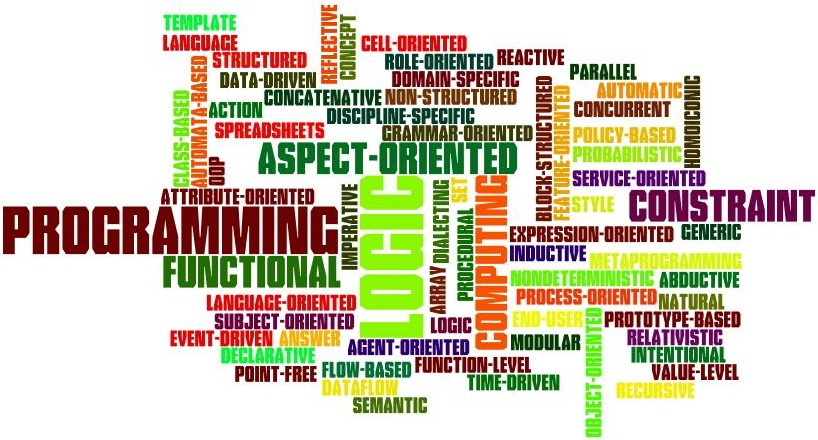
\includegraphics[width=1\textwidth]{programminglanguageparadigms.jpg} 
    \caption{Programming Paradigms}
 \end{figure}   
    \end{block}
    \end{column}
  \end{columns}
  \note[item]{}
\end{frame}

\begin{frame}
\frametitle{Classification}
  \begin{columns}[T]
    \begin{column}{.5\textwidth}
     \begin{block}{}
Programming languages are classified into paradigms depending on their characteristics and features. 
\\*For example, \textsc{Java} is an Object Oriented Programming Language.
    \end{block}
    \end{column}
    \begin{column}{.5\textwidth}
    \begin{block}{}
% Your image included here
\begin{figure}
    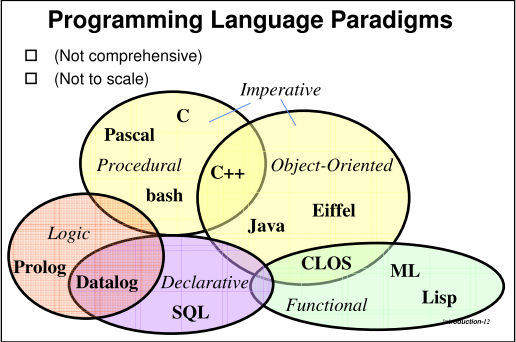
\includegraphics[width=\textwidth]{classification.png} 
    \caption{Classification of Programming Languages}
 \end{figure}   
    \end{block}
    \end{column}
  \end{columns}
  \note[item]{}
\end{frame}

\begin{frame}
\frametitle{Declarative Programming}
\begin{itemize}
\item Declarative style of programming.

These languages are said to describe (declaratively) what to do and not (operationally) how to do it.
\note[item]{http://www.eolss.net/sample-chapters/c15/e6-45-05-04.pdf}
\note[item]{One such style is the declarative paradigm, where the describe the logic of a computation without the control flow.[Practical 
Advantages of Declarative Programming Lloyd, J.W]}

\note[item]{It further branches out into functional and logic programming.}

\item For example, \progLang{Haskell}(functional language) and \progLang{Prolog}(logic language).
\note[item]{\progLang{Haskell} is a functional programming language while \progLang{Prolog} is a logic programming language.}
\note[item]{Both of them are declarative in nature but work differently.}

\end{itemize}
\end{frame}

\begin{frame}{Motivation}
\frametitle{(to be discarded ......)}
\begin{itemize}
\item Language classification.
\note[item]{Languages are classified into categories known paradigms depending on their characteristics.}
\note[item]{Languages from the same paradigm may exhibit different properties.} 

\item For example, \progLang{Haskell}(functional language) and \progLang{Prolog}(logic language).
\note[item]{\progLang{Haskell} is a functional programming language while \progLang{Prolog} is a logic programming language.}
\note[item]{Both of them are declarative in nature but work differently.}

\item Scope.
\note[item]{The versatility of a programming language is how well it can adapt to a particular problem.}
\note[item]{For instance, \progLang{Prolog} is good for rule based systems. "Clarissa", a voice user interface for browsing space station procedures is written in SICStus
	Prolog[https://ti.arc.nasa.gov/m/pub-archive/999h/0999\%20\%28Rayner\%29.pdf].}
\end{itemize}
\end{frame}

\begin{frame}{Scope}
	\note[item]{The versatility of a programming language is how well it can adapt to a particular problem.}
	\note[item]{For instance, \progLang{Prolog} is good for rule based systems. "Clarissa", a voice user interface for browsing space station procedures is written in SICStus
		Prolog[https://ti.arc.nasa.gov/m/pub-archive/999h/0999\%20\%28Rayner\%29.pdf].}
 \frametitle{General versus Special}
 \begin{columns}[T]
  \begin{column}{0.5\textwidth}
   \begin{block}{General Purpose Language}
    \textcolor{green}{Broad scope} but \textcolor{red}{problem needs to be moulded according to the capability of the language}.
    \note[item]{A truly general purpose programming language, GPL, is described which contains facilities for constructing (within the 
     language) new data types as well as facilities for operations performed upon them.[Jan V. Garwick. 1968. Programming Languages: GPL, a 
     truly general purpose language. Commun. ACM 11, 9 (September 1968), 634-638. DOI=http://dx.doi.org/10.1145/364063.364092]}
   \end{block}
  \end{column}

  \begin{column}{0.5\textwidth}
   \begin{block}{Special Purpose Language}
    \textcolor{red}{Limited scope} but \textcolor{green}{easier to express the problem as the suitable capabilities are readily available}. 
 	 \note[item]{A domain specific language is a concise micro language that offers tools and functionalities focused on solving problems 
 	 in a particular domain.} 
   \end{block}
  \end{column}
 \end{columns}
 
\end{frame}


\begin{frame}{Scope}
\frametitle{(to be discarded ......)}
\begin{itemize}
\item General purpose programming languages.
\note[item]{A truly general purpose programming language, GPL, is described which contains facilities for constructing (within the 
language) new data types as well as facilities for operations performed upon them.[Jan V. Garwick. 1968. Programming Languages: GPL, a 
truly general purpose language. Commun. ACM 11, 9 (September 1968), 634-638. DOI=http://dx.doi.org/10.1145/364063.364092]} 

\item Domain specific programming languages.
\note[item]{A domain specific language is a concise micro language that offers tools and functionalities focused on solving problems ona  
particular domain.} 
\end{itemize}
\end{frame}

\section{What was done}

\begin{frame}{Languages}
\begin{itemize}
\item Selection
\note[item]{Choosing a language is quite a daunting task. There are costs related to migration, training among others.}

\item Replicating functionality.
\note[item]{One option is to replicate the target language funcitonality in the current environment, and that is what we will look at 
today. Replicating \progLang{Prolog}-like functionality in \progLang{Haskell}}
\note[item]{The result is something close to a \textit{haskellised} \progLang{Prolog}, a functional eDSl with logic programming 
capabilities.}

\end{itemize}

\end{frame}

\clearpage

\begin{frame}{Background}

\begin{itemize}
\item Functional programming.
\note[item]{works by applying mathematical functions to arguments to get results. A program is not but functions which can also be passed 
to other functions as arguments.}

\item $\lambda$-calculi.
\note[item]{is a formal system in mathematical logic for expressing computations.}
\note[item]{The typed variant of $\lambda$-calculi puts restrictions on the type of data a function can work with.}

\item Damas-Hindley-Milner type system.
\note[item]{provides the ability to give a most general type to a function or program.}

\item For example, \progLang{Haskell}, \progLang{Scheme} and \progLang{Lisp}.
\end{itemize}
\end{frame}


\begin{frame}{Logic Programming}
\begin{itemize}
\item Logic programming.
\note[item]{is based on formal logic. A program consists of a set of rules used to derive a solution.}

\item Universal Horn clauses.
\note[item]{A Horn clause is a clause (a disjunction of literals) with at most one positive literal.}

\item For example, \progLang{Prolog}.
\end{itemize}
\end{frame}


\begin{frame}{Existing and Proposed Work}
\note[item]{Here we will look at the existing work,}
\begin{itemize}
\item Implementations.
\note[item]{Few exist. Incomplete and lack pratical features.}

\item Literature.
\note[item]{A series of papers provide useful insights into replicating \progLang{Prolog}-like clauses in \progLang{Haskell} though none
have accompanying implementations.}

\item Libraries.
\note[item]{Again a few exist and provide only a REPL interface. It is not possible to write a \progLang{Prolog}-like program in a file and
then compile and run it.}
\end{itemize}
\end{frame}

\begin{frame}{Improvements}
\note[item]{The improvements,}
\begin{itemize}
\item Practical features.
\note[item]{Firstly, we added practical features a \progLang{Prolog} distribution might, these being \prologConstruct{cut} and
\prologConstruct{fail}.}

\item \progLang{Prolog} in \progLang{Haskell}.
\note[item]{Meaning, one can write a program in our eDSl just like one would write a \progLang{Haskell} program.}
\end{itemize}
\end{frame}

\begin{frame}{Other Contributions}
\note[item]{In this section we will talk about, the contributions which are not neccessary an improvement on the current work but a new
direction for solving the problem of embedding languages.}
\begin{itemize}
\item Modular \textit{functorizing} mechanism.
\note[item]{We open up the language to accomodate meta syntactic variables, custom quantifiers and logic.}

\item Modular \textit{monadic} unification procedure.
\note[item]{this is to leverage imperative unification algorithms.}

\item Basic working \progLang{Prolog} implementation.
\note[item]{}

\item Variable search strategies.
\note[item]{Independent of how the solution search happens our implementation must work.}

\item Embedding IO in an eDSl. 
\note[item]{Modularizing the interpreter in a manner so that each stage must only deal with a particular aspect of the program.}

\end{itemize}
\end{frame}



\begin{frame}{Embedding a Programming Language into another Programming Language}
\note[item]{This section deals with embedding a target language in the host environement.}
\note[item]{The aim of this approach to bring the target language functionalities to the host language.}
\begin{itemize}
\item Embedding \progLang{Prolog}.
\note[item]{\progLang{Prolog} is a very popular choice for embedding.}

\item Target languages : \progLang{Java, Lisp, Scheme}.

\item \progLang{Prolog} in \progLang{Haskell} : \codeLibrary{Mini Prolog} and \codeLibrary{prolog}.
\note[item]{A \progLang{Prolog} implementation does exist for an older specification of \progLang{Haskell}.}

\item Logic programming in \progLang{Haskell}.
\note[item]{Few unification and backtracking libraries do exist for \progLang{Haskell} which use monads to capture and maintain state.}
\end{itemize}
\end{frame}





\begin{frame}{Multi Paradigm Languages (Functional Logic Languages)}
\note[item]{In this section we talk about languages that exhibit properties from multiple paradigms.}
\begin{itemize}
\item Multi paradigm language.
\note[item]{A multi-paradigm programming language is a programming language that supports more than one programming paradigm allowing the 
programmer to work in a variety of styles.[https://developer.mozilla.org/ar/docs/multiparadigmlanguage.html]}

\item For example, \progLang{Scala}.
\note[item]{A notable example is \progLang{Scala}, object functional language based on \progLang{Java}. Simply put it is Java with strong 
funcitonal characteristics such as higher order functions.}

\item Functional Logic programming languages.
\note[item]{are hybrid declarative languages exhibiting functional and logic programming languages.}

\item For example, \progLang{Curry}.
\note[item]{is a \progLang{Haskell} based functional logic programming language providing the choice operator for non deterministic
operations along with two way pattern matching.}

\item Other examples, \progLang{Mercury}.
\note[item]{which goes the other way round, starting from \progLang{Prolog} and adding \progLang{Haskell} features.}
\end{itemize}

\end{frame}



\begin{frame}{\progLang{Haskell}}
\begin{itemize}
\item
\end{itemize}

\end{frame}

\begin{frame}{\progLang{Prolog}}
\begin{itemize}
\item
\end{itemize}

\end{frame}


\begin{frame}{Related Concepts}
\begin{itemize}
\item
\end{itemize}

\end{frame}


\section{What we did}


\begin{frame}{Functorizing a language}
\begin{itemize}
\item
\end{itemize}

\end{frame}



\begin{frame}{Monadic unification}
\begin{itemize}
\item
\end{itemize}

\end{frame}


\subsection{Prototype 1}

\begin{frame}{Prototype 1}
\begin{figure}[H]
  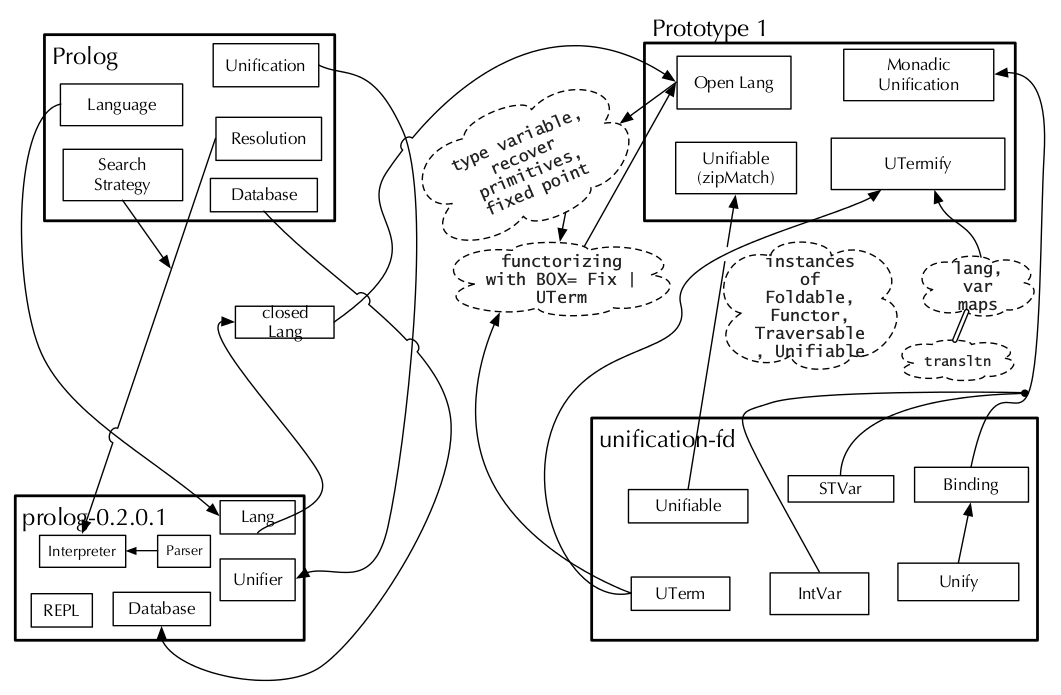
\includegraphics[width=1\textwidth]{Prototype-1-architecture.jpeg}
  \caption{Architecture of Prototype 1}
  \label{fig:proto1-arch}
\end{figure}
\end{frame}


\subsection{Prototype 2}
\begin{frame}{Prototype 2}
\begin{figure}[H]
  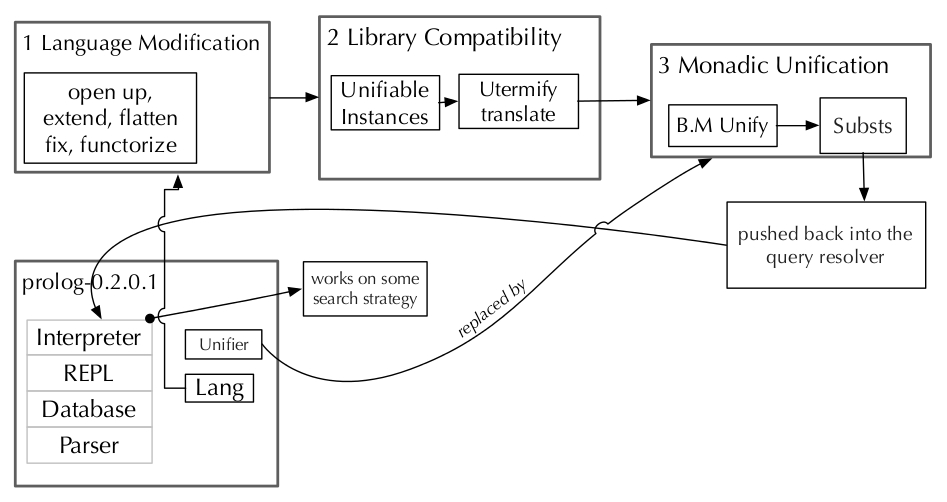
\includegraphics[width=1\textwidth]{Prototype-2-architecture.jpeg}
  \caption{Architecture of Prototype 2}
  \label{fig:proto1-arch}
\end{figure}

\end{frame}


\subsection{Prototype 3}

\begin{frame}{Prototype 3}
\begin{figure}[H]
  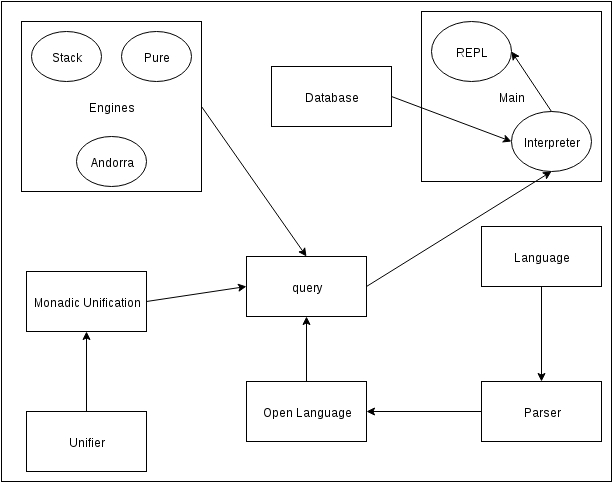
\includegraphics[width=0.75\textwidth]{Prototype-3-architecture.jpeg}
  \caption{Architecture of Prototype 3}
  \label{fig:proto1-arch}
\end{figure}
\end{frame}


\subsection{Prototype 4}

\begin{frame}{Prototype 4}
\begin{figure}[H]
  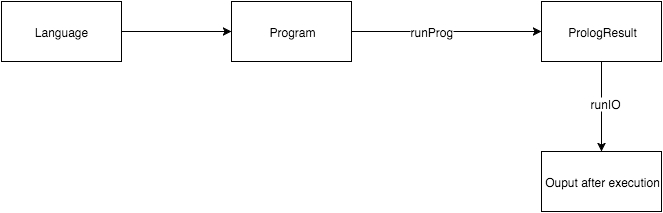
\includegraphics[width=1\textwidth]{Prototype-4-architecture.jpeg}
  \caption{Architecture of Prototype 4}
  \label{fig:proto1-arch}
\end{figure}
\end{frame}


\section{What remains to do}

\begin{frame}{Future Scope}
\begin{itemize}
\item
\end{itemize}

\end{frame}

\begin{frame}{Conclusion}
\begin{itemize}
\item
\end{itemize}

\end{frame}

\begin{frame}{The End}
\begin{center}
\Huge Questions?
\end{center}
\end{frame}


\section{Bibliography}
\begin{frame}[allowframebreaks]
	\frametitle{Bibliography}
	\setbeamertemplate{bibliography item}{[\theenumiv]}
	\nocite{*} 
	\bibliographystyle{plain} 
	\bibliography{Thesis-Presentation}
\end{frame}

\clearpage

%------------------------------------------------

\begin{frame}
\Huge{\centerline{The End}}
\end{frame}

%----------------------------------------------------------------------------------------

\end{document} 
